\documentclass[xcolor=svgnames]{beamer}\usepackage[]{graphicx}\usepackage[]{color}
%% maxwidth is the original width if it is less than linewidth
%% otherwise use linewidth (to make sure the graphics do not exceed the margin)
\makeatletter
\def\maxwidth{ %
  \ifdim\Gin@nat@width>\linewidth
    \linewidth
  \else
    \Gin@nat@width
  \fi
}
\makeatother

\definecolor{fgcolor}{rgb}{0.345, 0.345, 0.345}
\newcommand{\hlnum}[1]{\textcolor[rgb]{0.686,0.059,0.569}{#1}}%
\newcommand{\hlstr}[1]{\textcolor[rgb]{0.192,0.494,0.8}{#1}}%
\newcommand{\hlcom}[1]{\textcolor[rgb]{0.678,0.584,0.686}{\textit{#1}}}%
\newcommand{\hlopt}[1]{\textcolor[rgb]{0,0,0}{#1}}%
\newcommand{\hlstd}[1]{\textcolor[rgb]{0.345,0.345,0.345}{#1}}%
\newcommand{\hlkwa}[1]{\textcolor[rgb]{0.161,0.373,0.58}{\textbf{#1}}}%
\newcommand{\hlkwb}[1]{\textcolor[rgb]{0.69,0.353,0.396}{#1}}%
\newcommand{\hlkwc}[1]{\textcolor[rgb]{0.333,0.667,0.333}{#1}}%
\newcommand{\hlkwd}[1]{\textcolor[rgb]{0.737,0.353,0.396}{\textbf{#1}}}%

\usepackage{framed}
\makeatletter
\newenvironment{kframe}{%
 \def\at@end@of@kframe{}%
 \ifinner\ifhmode%
  \def\at@end@of@kframe{\end{minipage}}%
  \begin{minipage}{\columnwidth}%
 \fi\fi%
 \def\FrameCommand##1{\hskip\@totalleftmargin \hskip-\fboxsep
 \colorbox{shadecolor}{##1}\hskip-\fboxsep
     % There is no \\@totalrightmargin, so:
     \hskip-\linewidth \hskip-\@totalleftmargin \hskip\columnwidth}%
 \MakeFramed {\advance\hsize-\width
   \@totalleftmargin\z@ \linewidth\hsize
   \@setminipage}}%
 {\par\unskip\endMakeFramed%
 \at@end@of@kframe}
\makeatother

\definecolor{shadecolor}{rgb}{.97, .97, .97}
\definecolor{messagecolor}{rgb}{0, 0, 0}
\definecolor{warningcolor}{rgb}{1, 0, 1}
\definecolor{errorcolor}{rgb}{1, 0, 0}
\newenvironment{knitrout}{}{} % an empty environment to be redefined in TeX

\usepackage{alltt}
\usetheme{Boadilla}
\usecolortheme[named=SeaGreen]{structure}
\usepackage{graphicx}
\usepackage{breqn}
\usepackage{xcolor}
\usepackage{booktabs}
\usepackage{verbatim}
\usepackage{tikz}
\usepackage{lmodern}
\usetikzlibrary{shadows,arrows,positioning}
\definecolor{links}{HTML}{2A1B81}
\hypersetup{colorlinks,linkcolor=links,urlcolor=links}
\usepackage{pgfpages}

\newcommand{\Bigtxt}[1]{\textbf{\textit{#1}}}
\IfFileExists{upquote.sty}{\usepackage{upquote}}{}
\begin{document}

\title[Intro to EDA]{Introduction to exploratory data analysis}

\author[M. Beck, T. O'Brien]{Marcus W. Beck\inst{1} \and Todd D. O'Brien\inst{2}}

\date{}

\institute[]{\inst{1} ORISE, USEPA NHEERL Gulf Ecology Division\\ Email: \href{mailto:beck.marcus@epa.gov}{beck.marcus@epa.gov} \and \inst{2} NOAA/NMFS Copepod Project\\ Email: \href{todd.obrien@noaa.gov}{todd.obrien@noaa.gov}}

% knitr setup


% load SWMPr from local


%%%%%%
\begin{frame}
\vspace{0.3in}
\centerline{
\begin{tikzpicture}
  \node[drop shadow={shadow xshift=0ex,shadow yshift=0ex},fill=white,draw] at (0,0) {
\includegraphics[width=0.9\textwidth]{bg_main.jpg}};
\end{tikzpicture}}
\titlepage
\end{frame}

%%%%%%
\begin{frame}{Objectives and agenda}
\begin{itemize}
\onslide<+->
\item Objectives \\~\\
\begin{itemize}
\item What are some tools for pre-processing/organizing the SWMP data? \\~\\
\item What is the purpose of exploratory data analysis (EDA)? \\~\\
\item What are some common techniques and tools for EDA? \\~\\
\end{itemize}
\onslide<+->
\item Agenda \\~\\
\begin{itemize}
\item Organizing tools in SWMPr \\~\\
\item Purpose and overview of EDA \\~\\
\item Generic EDA tools in R, tools in SWMPr\\~\\
\end{itemize}
\end{itemize}
\end{frame}

%%%%%%
\begin{frame}{Interactive portion}
You can follow along in this module: \\~\\
\begin{itemize}
\item dataset2 \\~\\
\item script2 \\~\\
\end{itemize}
\Large
\centerline{\emph{Interactive! Interrupt me!}}
\end{frame}

%%%%%%
\begin{frame}{Import SWMP data and organize}
We learned how to import SWMP data in the previous session \\~\\
To review, the easiest approach is to download the data outside of R, then import using the `import_local' function \\~\\
Be sure that you use only the \href{http://cdmo.baruch.sc.edu/aqs/zips.cfm}{zip downloads} feature from CDMO - the `import_local' functions works best with these data \\~\\
\centerline{
\includegraphics[width = 0.8\textwidth]{adv_query.png}}
\end{frame}

%%%%%%
\begin{frame}[t]{Import SWMP data and organize}
It's best to download all the data possible for a reserve to avoid repeated requests to the server and to centralize the location from which the data are imported into R \\~\\
\centerline{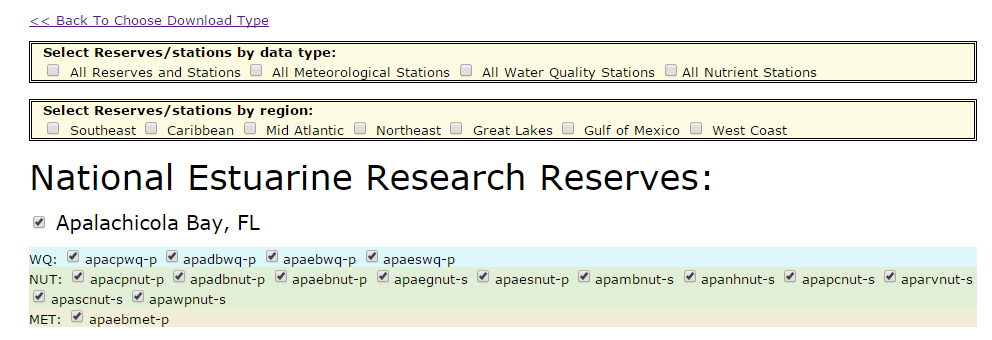
\includegraphics[width = \textwidth]{zip_eda.png}}
\end{frame}

%%%%%%
\begin{frame}[t]{Import SWMP data and organize}
It's best to download all the data possible for a reserve to avoid repeated requests to the server and to centralize the location from which the data are imported into R \\~\\
\centerline{
\includegraphics[width = 0.5\textwidth]{zip_eda2.png}}
Here we've made a request for all stations at Apalachicola Bay (water quality, nutrients, weather) and all available years (1995--2014) \\~\\
This request will take several minutes to be delivered to your email - an abbreviated version of these data are provided with the workshop materials for this training module
\end{frame}

%%%%%%
\begin{frame}[fragile]{Import SWMP data and organize}
Let's import some data for Apalachicola Bay

\begin{knitrout}\scriptsize
\definecolor{shadecolor}{rgb}{0.969, 0.969, 0.969}\color{fgcolor}\begin{kframe}
\begin{alltt}
\hlcom{# reload the SWMPr package just in case}
\hlkwd{library}\hlstd{(SWMPr)}

\hlcom{# import data}
\hlcom{# change this path for the flash drive}
\hlstd{path} \hlkwb{<-} \hlstr{'C:/data/dataset2'}
\hlstd{wq_dat} \hlkwb{<-} \hlkwd{import_local}\hlstd{(path,} \hlstr{'apacpwq'}\hlstd{)}
\hlstd{nut_dat} \hlkwb{<-} \hlkwd{import_local}\hlstd{(path,} \hlstr{'apacpnut'}\hlstd{)}
\hlstd{met_dat} \hlkwb{<-} \hlkwd{import_local}\hlstd{(path,} \hlstr{'apaebmet'}\hlstd{)}
\end{alltt}
\end{kframe}
\end{knitrout}
We've just imported data from 2011--2014 for three stations (apacpwq, apacpnut, apaebmet) and saved them in our workspace as three separate objects (wq_dat, nut_dat, met_dat)
\end{frame}

%%%%%%
\begin{frame}[fragile]{Import SWMP data and organize}
But don't take my word for it, take a look at the data!
\begin{knitrout}\scriptsize
\definecolor{shadecolor}{rgb}{0.969, 0.969, 0.969}\color{fgcolor}\begin{kframe}
\begin{alltt}
\hlcom{# what are the dimenions of the water quality data?}
\hlkwd{dim}\hlstd{(wq_dat)}
\end{alltt}
\begin{verbatim}
## [1] 132035     25
\end{verbatim}
\begin{alltt}
\hlcom{# what are the dimenions of the nutrient data?}
\hlkwd{dim}\hlstd{(nut_dat)}
\end{alltt}
\begin{verbatim}
## [1] 48 13
\end{verbatim}
\begin{alltt}
\hlcom{# what are the dimenions of the weather data?}
\hlkwd{dim}\hlstd{(met_dat)}
\end{alltt}
\begin{verbatim}
## [1] 133548     23
\end{verbatim}
\end{kframe}
\end{knitrout}
\end{frame}

%%%%%%
\begin{frame}[fragile,shrink]{Import SWMP data and organize}
View the first six rows
\begin{knitrout}\scriptsize
\definecolor{shadecolor}{rgb}{0.969, 0.969, 0.969}\color{fgcolor}\begin{kframe}
\begin{alltt}
\hlcom{# View the first six rows of the wq data}
\hlkwd{head}\hlstd{(wq_dat)}
\end{alltt}
\begin{verbatim}
##         datetimestamp temp f_temp spcond f_spcond sal f_sal do_pct f_do_pct
## 1 2011-01-01 00:00:00   11   <0>      44     <0>   28  <0>      68     <0> 
## 2 2011-01-01 00:15:00   11   <0>      44     <0>   28  <0>      68     <0> 
## 3 2011-01-01 00:30:00   11   <0>      44     <0>   28  <0>      68     <0> 
## 4 2011-01-01 00:45:00   11   <0>      44     <0>   28  <0>      68     <0> 
## 5 2011-01-01 01:00:00   11   <0>      44     <0>   29  <0>      68     <0> 
## 6 2011-01-01 01:15:00   11   <0>      44     <0>   29  <0>      67     <0> 
##   do_mgl f_do_mgl depth f_depth cdepth f_cdepth level f_level clevel f_clevel
## 1      6     <0>      2    <0>       2     <3>     NA   <-1>      NA       NA
## 2      6     <0>      2    <0>       2     <3>     NA   <-1>      NA       NA
## 3      6     <0>      2    <0>       2     <3>     NA   <-1>      NA       NA
## 4      6     <0>      2    <0>       2     <3>     NA   <-1>      NA       NA
## 5      6     <0>      2    <0>       2     <3>     NA   <-1>      NA       NA
## 6      6     <0>      2    <0>       2     <3>     NA   <-1>      NA       NA
##   ph f_ph turb f_turb chlfluor f_chlfluor
## 1  8 <0>     3   <0>        NA      <-1> 
## 2  8 <0>     3   <0>        NA      <-1> 
## 3  8 <0>     2   <0>        NA      <-1> 
## 4  8 <0>     1   <0>        NA      <-1> 
## 5  8 <0>     2   <0>        NA      <-1> 
## 6  8 <0>     1   <0>        NA      <-1>
\end{verbatim}
\end{kframe}
\end{knitrout}
\end{frame}

%%%%%%
\begin{frame}[fragile,shrink]{Import SWMP data and organize}
View the last six rows
\begin{knitrout}\scriptsize
\definecolor{shadecolor}{rgb}{0.969, 0.969, 0.969}\color{fgcolor}\begin{kframe}
\begin{alltt}
\hlcom{# View the last six rows of the wq data}
\hlkwd{tail}\hlstd{(wq_dat)}
\end{alltt}
\begin{verbatim}
##              datetimestamp temp f_temp spcond f_spcond sal f_sal do_pct
## 132030 2014-10-07 07:45:00   24   <0>      41     <0>   26  <0>      90
## 132031 2014-10-07 08:00:00   24   <0>      41     <0>   26  <0>      91
## 132032 2014-10-07 08:15:00   23   <0>      39     <0>   25  <0>      95
## 132033 2014-10-07 08:30:00   23   <0>      39     <0>   25  <0>      95
## 132034 2014-10-07 08:45:00   24   <0>      38     <0>   24  <0>      95
## 132035 2014-10-07 09:00:00   24   <0>      38     <0>   24  <0>      96
##        f_do_pct do_mgl f_do_mgl depth f_depth cdepth f_cdepth level f_level
## 132030     <0>       7     <0>      2    <0>       2     <3>     NA   <-1> 
## 132031     <0>       7     <0>      2    <0>       2     <3>     NA   <-1> 
## 132032     <0>       7     <0>      2    <0>       2     <3>     NA   <-1> 
## 132033     <0>       7     <0>      2    <0>       2     <3>     NA   <-1> 
## 132034     <0>       7     <0>      2    <0>       2     <3>     NA   <-1> 
## 132035     <0>       7     <0>      2    <0>       2     <3>     NA   <-1> 
##        clevel f_clevel ph f_ph turb f_turb chlfluor f_chlfluor
## 132030     NA       NA  8 <0>    10   <0>        NA      <-1> 
## 132031     NA       NA  8 <0>     8   <0>        NA      <-1> 
## 132032     NA       NA  8 <0>     7   <0>        NA      <-1> 
## 132033     NA       NA  8 <0>     7   <0>        NA      <-1> 
## 132034     NA       NA  8 <0>     7   <0>        NA      <-1> 
## 132035     NA       NA  8 <0>     5   <0>        NA      <-1>
\end{verbatim}
\end{kframe}
\end{knitrout}
\end{frame}

%%%%%%
\begin{frame}[fragile,shrink]{Import SWMP data and organize}
What class is the data?
\begin{knitrout}\scriptsize
\definecolor{shadecolor}{rgb}{0.969, 0.969, 0.969}\color{fgcolor}\begin{kframe}
\begin{alltt}
\hlcom{# class of the data}
\hlkwd{class}\hlstd{(wq_dat)}
\end{alltt}
\begin{verbatim}
## [1] "swmpr"      "data.frame"
\end{verbatim}
\end{kframe}
\end{knitrout}
This tells us that the imported data are two different classes - `swmpr' and `data.frame'\\~\\
The class of an object is important because it defines the types of methods (i.e., functions) that apply\\~\\
For example, `head' and `tail' functions apply to a `data.frame'
\end{frame}

%%%%%%
\begin{frame}[fragile,shrink]{Import SWMP data and organize}
The swmpr object class was developed to make your life easier working with SWMP data, i.e., functions in the SWMPr package organize and analyze raw SWMP data\\~\\
The \href{https://github.com/fawda123/SWMPr}{online documentation} describes the functions that work with the swmpr object class, also...
\begin{knitrout}\scriptsize
\definecolor{shadecolor}{rgb}{0.969, 0.969, 0.969}\color{fgcolor}\begin{kframe}
\begin{alltt}
\hlcom{# what functions/methods work with swmpr objects?}
\hlkwd{methods}\hlstd{(}\hlkwc{class} \hlstd{=} \hlstr{'swmpr'}\hlstd{)}
\end{alltt}
\begin{verbatim}
##  [1] aggregate.swmpr comb.swmpr      decomp.swmpr    hist.swmpr     
##  [5] lines.swmpr     na.approx.swmpr plot.swmpr      qaqc.swmpr     
##  [9] qaqcchk.swmpr   setstep.swmpr   smoother.swmpr  subset.swmpr
\end{verbatim}
\end{kframe}
\end{knitrout}
Documentation of each function can be viewed as follows (although currently not complete):
\begin{knitrout}\scriptsize
\definecolor{shadecolor}{rgb}{0.969, 0.969, 0.969}\color{fgcolor}\begin{kframe}
\begin{alltt}
\hlcom{# see help for a swmpr function}
\hlopt{?}\hlstd{aggregate.swmpr}

\hlcom{# or...}
\hlkwd{help}\hlstd{(}\hlstr{'aggregate.swmpr'}\hlstd{)}
\end{alltt}
\end{kframe}
\end{knitrout}
\end{frame}

%%%%%
\begin{frame}[fragile,shrink]{Import SWMP data and organize}
A useful feature of R is that a defined class will have both \Bigtxt{data} and \Bigtxt{attributes}\\~\\
For the swmpr object class, the \Bigtxt{data} are the raw swmpr data as a data.frame \\~\\
The \Bigtxt{attributes} are a list of metadata for the imported data
\begin{knitrout}\scriptsize
\definecolor{shadecolor}{rgb}{0.969, 0.969, 0.969}\color{fgcolor}\begin{kframe}
\begin{alltt}
\hlcom{# what attributes are available for a swmpr object}
\hlkwd{names}\hlstd{(}\hlkwd{attributes}\hlstd{(wq_dat))}
\end{alltt}
\begin{verbatim}
## [1] "names"       "row.names"   "class"       "station"     "parameters" 
## [6] "qaqc_cols"   "date_rng"    "timezone"    "stamp_class"
\end{verbatim}
\begin{alltt}
\hlcom{# view the parameters}
\hlkwd{attr}\hlstd{(wq_dat,} \hlstr{'parameters'}\hlstd{)}
\end{alltt}
\begin{verbatim}
##  [1] "temp"     "spcond"   "sal"      "do_pct"   "do_mgl"   "depth"   
##  [7] "cdepth"   "level"    "clevel"   "ph"       "turb"     "chlfluor"
\end{verbatim}
\end{kframe}
\end{knitrout}
\end{frame}

%%%%%
\begin{frame}[fragile]{Import SWMP data and organize}
You can also view all the attributes as follows:
\begin{knitrout}\scriptsize
\definecolor{shadecolor}{rgb}{0.969, 0.969, 0.969}\color{fgcolor}\begin{kframe}
\begin{alltt}
\hlcom{# view all attributes}
\hlkwd{attributes}\hlstd{(wq_dat)}
\end{alltt}
\end{kframe}
\end{knitrout}
This is not recommended since they are quite long, e.g., an attribute of the `data.frame' class is the row names (132035 rows for`wq\_dat') \\~\\
Individual attributes are useful for getting a feel for the dataset - what is the date range? what parameters are included? are QAQC columns present? \\~\\
However, the intended use of attributes is behind the scenes with swmpr functions - they will be used to process the data and updated automatically
\end{frame}

%%%%%%
\begin{frame}[fragile,shrink]{Import SWMP data and organize}
Now that we have a feel for the data, what needs to be done before we can start analyzing the information? \\~\\
Last module: \\~\\
\begin{itemize}
\item How do we handle QAQC data or `bad' observations?
\item How do we deal with data we don't want?  
\item How do we combine data for comparison?
\item How do we handle issues inherent with time series? \\~\\
\end{itemize}
Several of these problems are context-dependent - driven by the question or analysis \\~\\
Others are common to any analysis...
\end{frame}

%%%%%%
\begin{frame}[fragile]{Import SWMP data and organize}
Perhaps the first organizational tool you want to use is `qaqc.swmpr'\\~\\
This function does two things:\\~\\
\begin{itemize}
\item Remove observations with a specified QAQC flag value
\item Remove extraneous QAQC columns \\~\\
\end{itemize}
\centerline{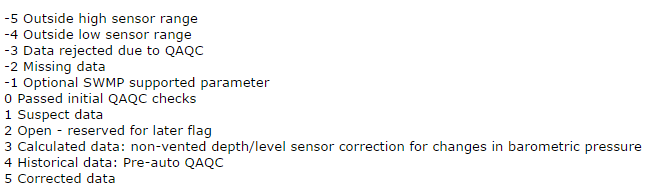
\includegraphics[width = 0.8\textwidth]{qaqc_flags.png}}
\end{frame}

%%%%%%
\begin{frame}[fragile]{Import SWMP data and organize}
You will have to decide which values to keep - be conservative and only keep those that passed QAQC (best option?) or keep all the data (worst option?) \\~\\
To help you decide, it may be useful to get an idea of the distribution of QAQC flags in the data\\~\\
\begin{knitrout}\scriptsize
\definecolor{shadecolor}{rgb}{0.969, 0.969, 0.969}\color{fgcolor}\begin{kframe}
\begin{alltt}
\hlcom{# use qaqcchk to view distributin of qaqc flags}
\hlstd{myqaqc} \hlkwb{<-} \hlkwd{qaqcchk}\hlstd{(wq_dat)}

\hlcom{# view first six rows}
\hlkwd{head}\hlstd{(myqaqc)}
\end{alltt}
\begin{verbatim}
##        piece f_cdepth f_chlfluor f_depth f_do_mgl f_do_pct f_level f_ph f_sal
## 1                 288         NA      NA       NA       NA      NA   NA    NA
## 2      <-1>        NA     132035      NA       NA       NA  132035   NA    NA
## 3 <-1> [GCU]        9         NA      NA       NA       NA      NA   NA    NA
## 4      <-2>        NA         NA      90       90       90      NA   90    90
## 5 <-2> (CSM)       NA         NA      51       51       51      NA   51    51
## 6 <-2> [GCM]     1353         NA      NA       NA       NA      NA   NA    NA
##   f_spcond f_temp f_turb
## 1       NA     NA     NA
## 2       NA     NA     NA
## 3       NA     NA     NA
## 4       90     90     90
## 5       51     51     51
## 6       NA     NA     NA
\end{verbatim}
\end{kframe}
\end{knitrout}
\end{frame}

%%%%%%
\begin{frame}
\vspace{0.3in}
\centerline{
\begin{tikzpicture}
  \node[drop shadow={shadow xshift=0ex,shadow yshift=0ex},fill=white,draw] at (0,0) {
\includegraphics[width=0.9\textwidth]{bg_main.jpg}};
\end{tikzpicture}}
\vspace{0.5in}
\Large
\centerline{\Bigtxt{Questions??}}
\end{frame}

\end{document}
